% Furrows & DFH experiments — Hunter on agricultural soil
% Compile: pdflatex furrows_dfh_experiments.tex   (run twice for refs)
\documentclass[aspectratio=169,10pt]{beamer}

\usetheme{Madrid}
\usecolortheme{seahorse}
\useinnertheme{circles}
\setbeamertemplate{navigation symbols}{}
\setbeamertemplate{footline}[frame number]

\usepackage{booktabs}
\usepackage{array}
\usepackage{xcolor}
\usepackage{graphicx}
\graphicspath{{figs/}}

\definecolor{good}{RGB}{30,130,60}
\definecolor{bad}{RGB}{190,40,40}
\newcommand{\yes}{\textcolor{good}{\textbf{works}}}
\newcommand{\no}{\textcolor{bad}{\textbf{null}}}

\title[Furrows \& DFH]{Walking the Hunter Biped on Agricultural Soil}
\subtitle{Two experiments: rigid furrows (deploys) vs.\ deformable soil (a clean null)}
\author{HumanoidVerse $\cdot$ Hunter $\cdot$ IsaacSim/IsaacLab}
\date{\today}

\begin{document}

\begin{frame}[plain]
  \titlepage
\end{frame}

% ---------------------------------------------------------------
\begin{frame}{The question, in one slide}
  \textbf{Goal:} make the Hunter biped walk across a tilled crop field in simulation,
  robustly enough to deploy.

  \vspace{1em}
  We ran \alert{two separate experiments}, each asking a different question:

  \vspace{0.8em}
  \begin{columns}[T]
    \begin{column}{0.48\textwidth}
      \begin{block}{1.\ Furrows (geometry)}
        Can the robot handle the \emph{shape} of plowed ground --- ridges and
        grooves --- if the ground is still \emph{rigid}?
        \\[0.4em]
        \textbf{Answer: \yes} --- produced the policies we deploy.
      \end{block}
    \end{column}
    \begin{column}{0.48\textwidth}
      \begin{block}{2.\ DFH (deformable soil)}
        Does adding \emph{soft, sinking, dragging} soil physics make a
        \emph{measurably better} walker than rigid training?
        \\[0.4em]
        \textbf{Answer: \no} --- soil-trained did not beat rigid-trained.
      \end{block}
    \end{column}
  \end{columns}

  \vspace{1em}
  \footnotesize Both share the same robot (Hunter), simulator (IsaacSim 4.2),
  and algorithm (PPO-ROA, 234-dim history observation).
\end{frame}

% ===============================================================
\section{Experiment 1 --- Furrows}

\begin{frame}{Experiment 1: Furrows --- what is being tested}
  A \textbf{furrow} = the groove + crest pattern left by plowing.
  We bake that shape into a \emph{rigid} heightfield and ask the robot to
  walk across the rows.

  \vspace{0.6em}
  \begin{itemize}
    \item Ground is hard (friction $\mu_s{=}0.60$, $\mu_d{=}0.45$); only the
          \alert{geometry} is hard, not the material.
    \item Trained as a \textbf{3-stage curriculum} --- start easy, promote when
          stable, then harden the terrain.
  \end{itemize}

  \vspace{0.6em}
  \begin{center}
  \begin{tabular}{lcccc}
    \toprule
    Stage & Groove depth & Row spacing & Row tilt & Crest lift \\
    \midrule
    1 Easy   & 0.08--0.12\,m & 2.7--3.2\,m & $0^\circ$           & 0.05\,m \\
    2 Medium & 0.15--0.20\,m & 2.0--2.5\,m & $\pm 3^\circ$       & 0.03\,m \\
    3 Full   & 0.20--0.30\,m & 1.5--2.0\,m & $\pm 5^\circ$       & 0.00\,m \\
    \bottomrule
  \end{tabular}
  \end{center}

  \vspace{0.4em}
  \footnotesize Each stage = deeper grooves, tighter rows, more misalignment ---
  i.e.\ progressively harder footing.
\end{frame}

\begin{frame}{Experiment 1: promotion rule \& result}
  \textbf{We only advance a stage when the policy is genuinely stable:}
  \begin{center}
  \begin{tabular}{lll}
    \toprule
    Promotion & Episode length & Termination reward \\
    \midrule
    Stage 1 $\rightarrow$ 2 & $\geq 16$\,s & $\geq -0.05$/s \\
    Stage 2 $\rightarrow$ 3 & $\geq 18$\,s & $\geq -0.03$/s \;(+ real gait) \\
    Stage 3 target          & $\sim$19--20\,s & stable tracking \\
    \bottomrule
  \end{tabular}
  \end{center}

  \vspace{0.8em}
  \begin{block}{Outcome \yes}
    The furrows curriculum produced the \textbf{working walkers we ship}:
    \begin{itemize}
      \item \texttt{v7\_baseline} --- flat-ground walker (warm-start root)
      \item \texttt{rigid\_walker} --- walks rigid furrows
      \item \texttt{mildsoil\_walker} (\texttt{model\_5050}) --- \alert{deployment policy},
            velocity error 0.098, drives the agri-field demo
    \end{itemize}
    All published to HuggingFace (\texttt{anhrisn/hunter-dfh-locomotion}).
  \end{block}
\end{frame}

\begin{frame}{Experiment 1: does it actually learn? (yes)}
  Two signals, read straight off the training logs of the deployment model:
  \begin{center}
    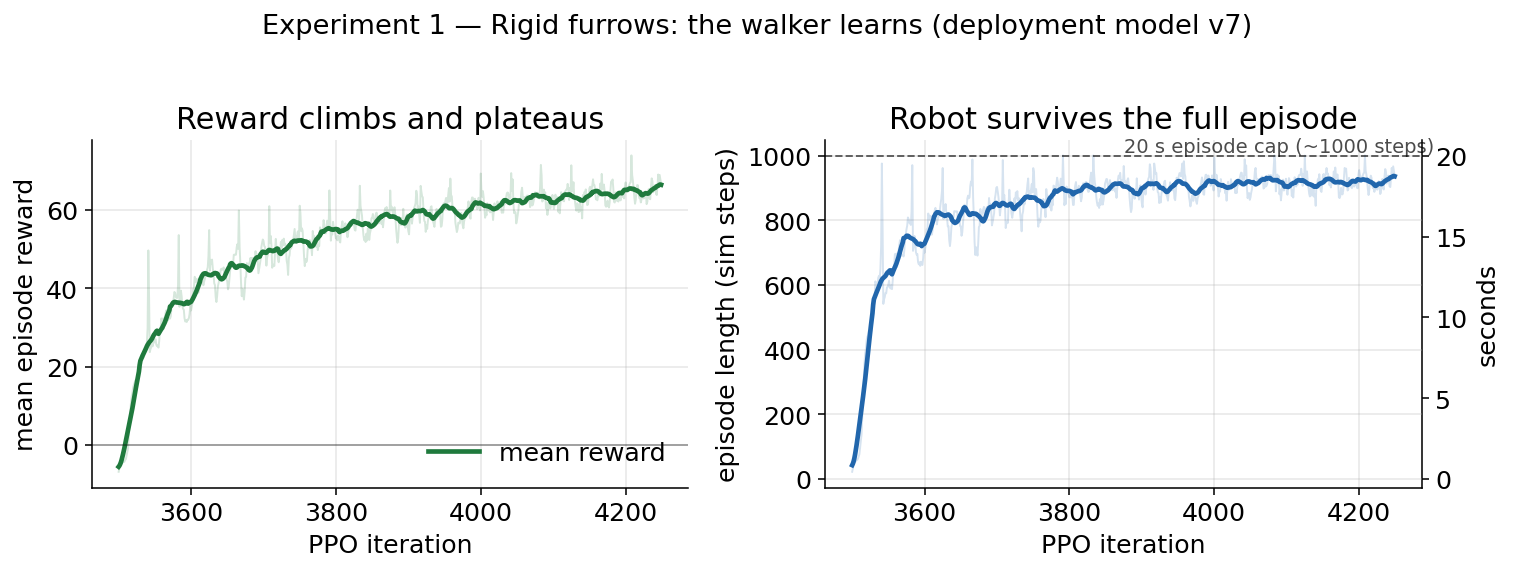
\includegraphics[width=0.80\textwidth]{fig1_furrows_learn.png}
  \end{center}
  \vspace{-0.3em}
  \begin{itemize}\footnotesize
    \item \textbf{Left:} mean reward rises from below zero and \emph{plateaus high}
          --- a healthy PPO curve.
    \item \textbf{Right:} episode length climbs to near the \textbf{20\,s cap}
          ($\sim$1000 steps) --- the robot survives the whole episode.
    \item \alert{Reward up + episodes long = it learned to walk}, not just to stand.
  \end{itemize}
\end{frame}

\begin{frame}{Which rewards actually drove the learning?}
  The total reward is a sum of \textbf{17 terms}. Breaking the final policy apart
  shows what the robot is really being paid for:
  \begin{center}
    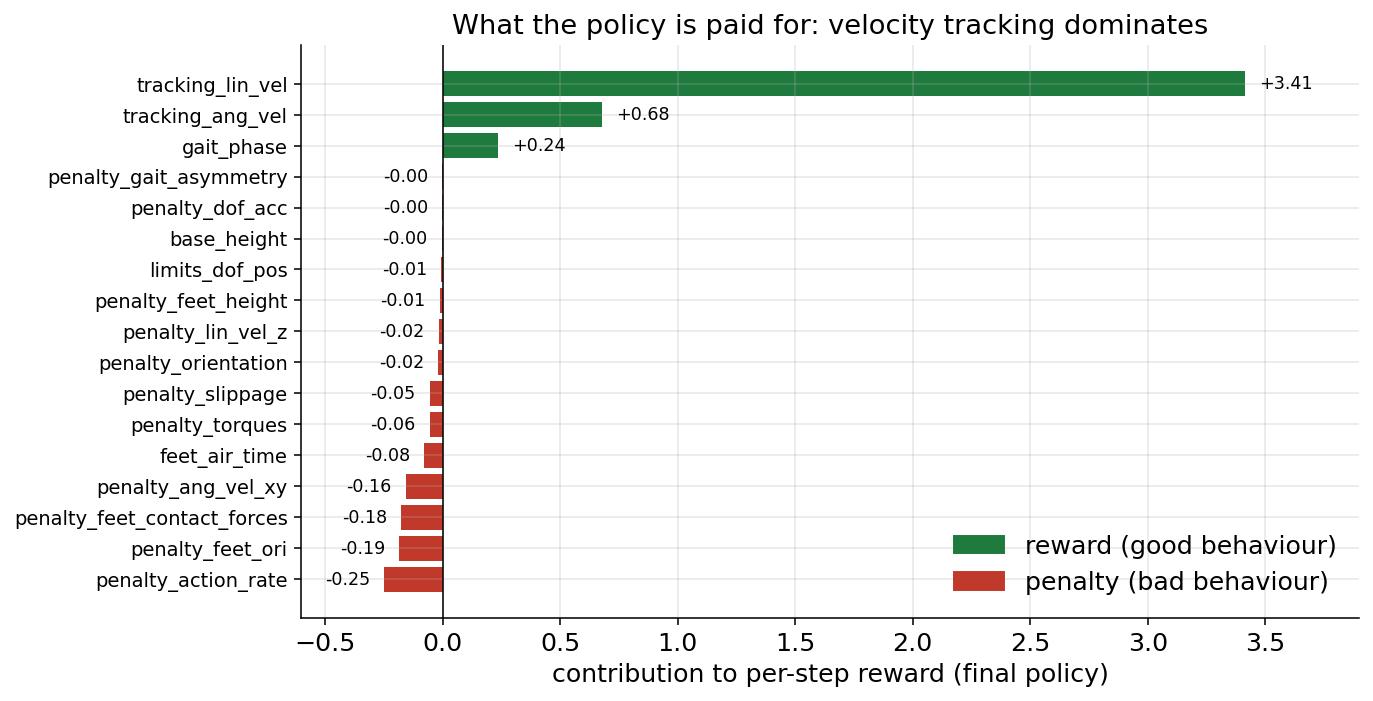
\includegraphics[width=0.58\textwidth]{fig5_reward_budget.png}
  \end{center}
  \vspace{-0.3em}
  \begin{itemize}\footnotesize
    \item \alert{Velocity tracking} (\texttt{tracking\_lin\_vel}, $+3.41$) dwarfs
          everything --- ``go at the commanded speed'' is the goal that pulls the
          policy.
    \item \texttt{tracking\_ang\_vel} ($+0.68$) and \texttt{gait\_phase} ($+0.24$)
          shape \emph{turning} and a \emph{rhythmic gait}.
    \item All penalties (red) stay \textbf{small} --- they tidy up the motion
          (smooth actions, gentle contacts) without overpowering the goal.
  \end{itemize}
\end{frame}

\begin{frame}{Same story, over time: tracking is the engine}
  \begin{center}
    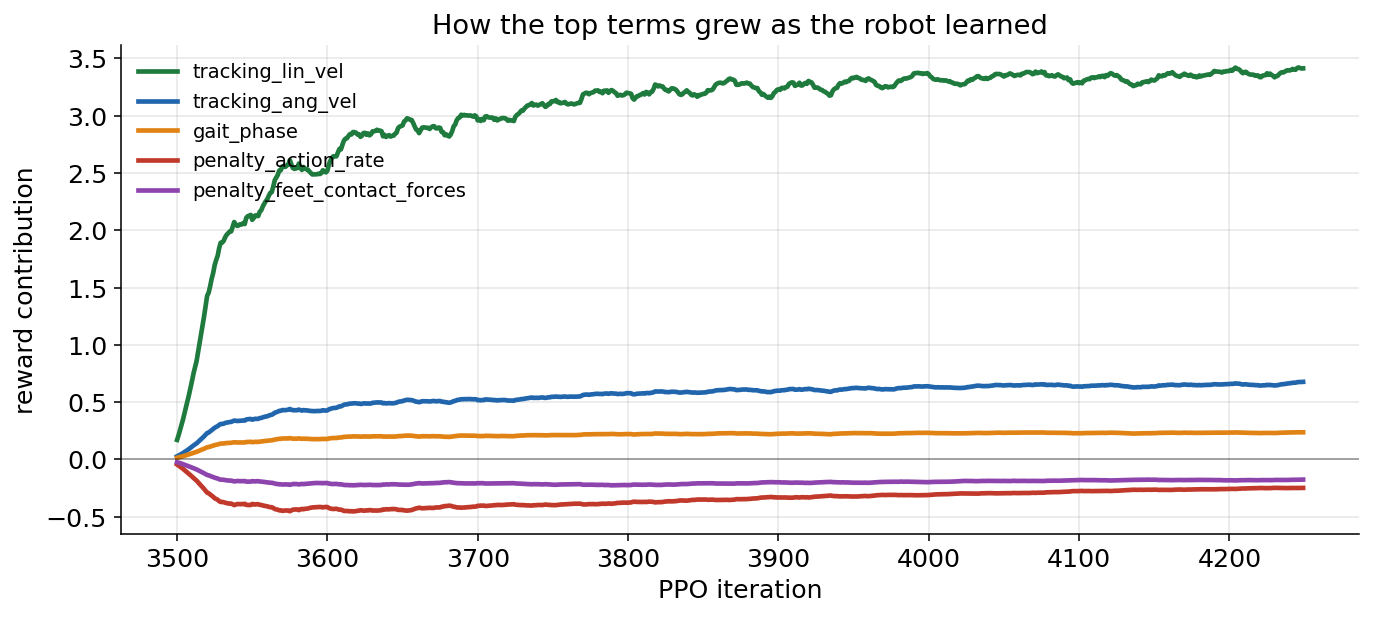
\includegraphics[width=0.72\textwidth]{fig6_reward_growth.png}
  \end{center}
  \vspace{-0.3em}
  \begin{itemize}\footnotesize
    \item The green \texttt{tracking\_lin\_vel} curve has \alert{the same shape as the
          total-reward curve} --- it \emph{is} what drove the climb.
    \item Gait and turning rewards grow gently, then settle into a stable rhythm.
    \item Penalties (red/purple) deepen only slightly --- the cost of moving faster,
          not a fight against the reward.
    \item \textbf{Takeaway:} learning $=$ ``chase the velocity command cleanly''; the
          other 16 terms are guardrails, not the driver.
  \end{itemize}
\end{frame}

% ===============================================================
\section{Experiment 2 --- DFH}

\begin{frame}{Experiment 2: DFH --- adding real soil physics}
  \textbf{DFH = Deformable Furrowed Heightfield.} On top of the furrow shape, the
  ground now \emph{responds} to the feet. Five physical effects, all GPU-resident:

  \vspace{0.5em}
  \begin{columns}[T]
    \begin{column}{0.55\textwidth}
      \begin{enumerate}
        \item \textbf{Sinkage} (Bekker): feet press in under load.
        \item \textbf{Slip-sinkage} (Wong--Reece): a dragging foot digs deeper.
        \item \textbf{Plastic ratchet}: a dent stays dented within an episode.
        \item \textbf{Bulldozing}: pushed soil rises in neighbour cells.
        \item \textbf{Anisotropic friction}: harder to slide \emph{across} rows
              than \emph{along} them.
      \end{enumerate}
    \end{column}
    \begin{column}{0.43\textwidth}
      \begin{block}{The force on the robot}
        Each foot feels a tangential drag:
        \[
          F_{\text{drag}} = k \cdot \text{sinkage} \cdot F_{\text{normal}}
        \]
        clamped at \texttt{max\_drag\_force\_n}.
        \\[0.4em]
        \footnotesize Deeper sink $\Rightarrow$ more drag $\Rightarrow$ the robot
        must actively fight the soil.
      \end{block}
    \end{column}
  \end{columns}

  \vspace{0.4em}
  \footnotesize Difficulty rises with the curriculum: softer soil (lower Bekker
  moduli), wider anisotropy, deeper sink cap (5\,cm $\rightarrow$ 10\,cm).
\end{frame}

\begin{frame}{Experiment 2: a fair test --- the paired protocol}
  To claim ``soil training helps'' we must beat the obvious baseline. So for each
  random seed we trained \alert{three matched policies}:

  \vspace{0.5em}
  \begin{center}
  \begin{tabular}{ll}
    \toprule
    Policy & Trained on \\
    \midrule
    \textbf{RIGID}    & rigid furrows (no soil forces) --- the baseline \\
    \textbf{SHADOW}   & soil computed but \emph{forces off} (sanity check) \\
    \textbf{DFH\_FULL}& soil + drag forces active \\
    \bottomrule
  \end{tabular}
  \end{center}

  \vspace{0.7em}
  All three are then evaluated \emph{on the same deformable terrain}. The headline
  number is the \textbf{paired regret}:
  \[
    \text{regret} = \text{ep\_len}(\textsf{DFH\_FULL}@\text{soil}) -
                    \text{ep\_len}(\textsf{RIGID}@\text{soil})
  \]
  \begin{itemize}\footnotesize
    \item \textbf{Positive} regret $\Rightarrow$ soil training paid off.
    \item Reward shaping for sink held at \textbf{zero} during the test, so any
          gain is from \emph{dynamics}, not hand-tuned rewards.
    \item Success bar set \emph{in advance}: drag 5--10\% body weight, regret $>0$
          on every seed, mean regret $\geq 10\%$ of baseline.
  \end{itemize}
\end{frame}

\begin{frame}{Experiment 2: both policies learn (this is not a training failure)}
  \footnotesize
  \textbf{RIGID} = trained on the \emph{rigid furrowed heightfield} --- the hard,
  plowed-shape ground from Experiment 1 (geometry only, the surface never moves).
  \textbf{SOIL (DFH)} = the \emph{same} furrows, but the ground now sinks, drags and
  deforms. So ``rigid'' is the furrow heightfield with the soil physics switched off.
  \begin{center}
    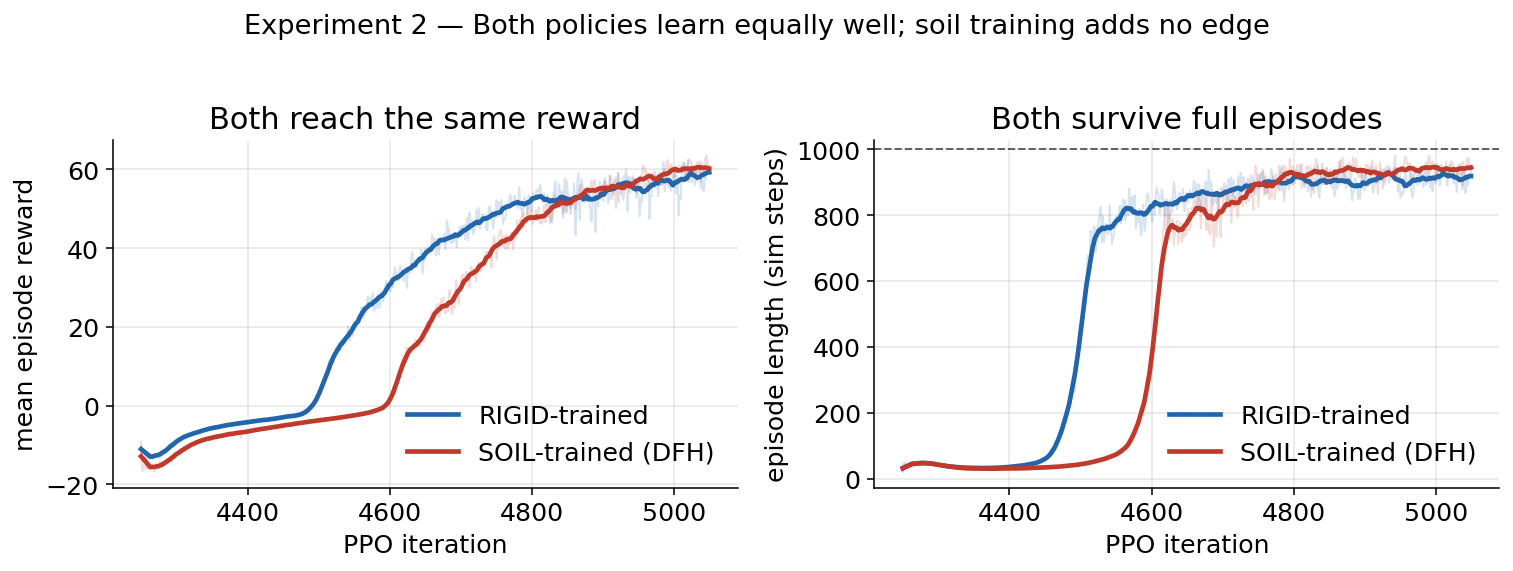
\includegraphics[width=0.88\textwidth]{fig2_paired_learn.png}
  \end{center}
  \begin{itemize}\footnotesize
    \item Both climb to the \textbf{same reward} ($\sim$60) and \textbf{same episode
          length} ($\sim$1000 steps).
    \item The soil-trained one takes off a bit later (it fights drag) but
          \alert{catches up completely} --- so any later gap is \emph{not} a training
          failure.
  \end{itemize}
\end{frame}

\begin{frame}{Experiment 2: the soil load is real --- and it copes}
  \footnotesize
  \textbf{Drag as \% of body weight} = the backward pull the soil puts on the feet,
  divided by the robot's own weight. We normalise by weight so the number is
  intuitive and robot-independent: ``10\%'' means the soil resists with a force equal
  to one-tenth of the robot --- like wading through mud. It is our honest measure of
  \emph{how hard the terrain is fighting the robot}.
  \begin{center}
    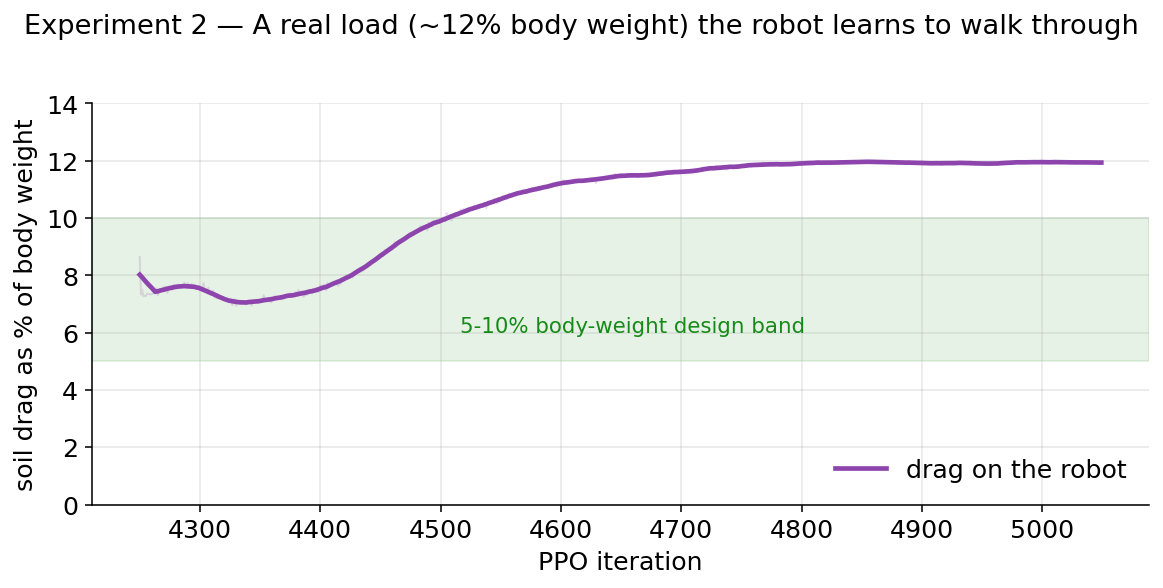
\includegraphics[width=0.72\textwidth]{fig3_drag_budget.png}
  \end{center}
  \vspace{-0.3em}
  \begin{itemize}\footnotesize
    \item Settles at $\sim$\textbf{12\% body weight} --- a genuine, persistent load,
          in the range we designed for.
    \item Episodes still reach the cap, so the robot \alert{learned to walk through
          that drag}: the physics is doing real work on it.
  \end{itemize}
\end{frame}

\begin{frame}{Experiment 2: why the harder soil stages are brutal}
  \begin{center}
    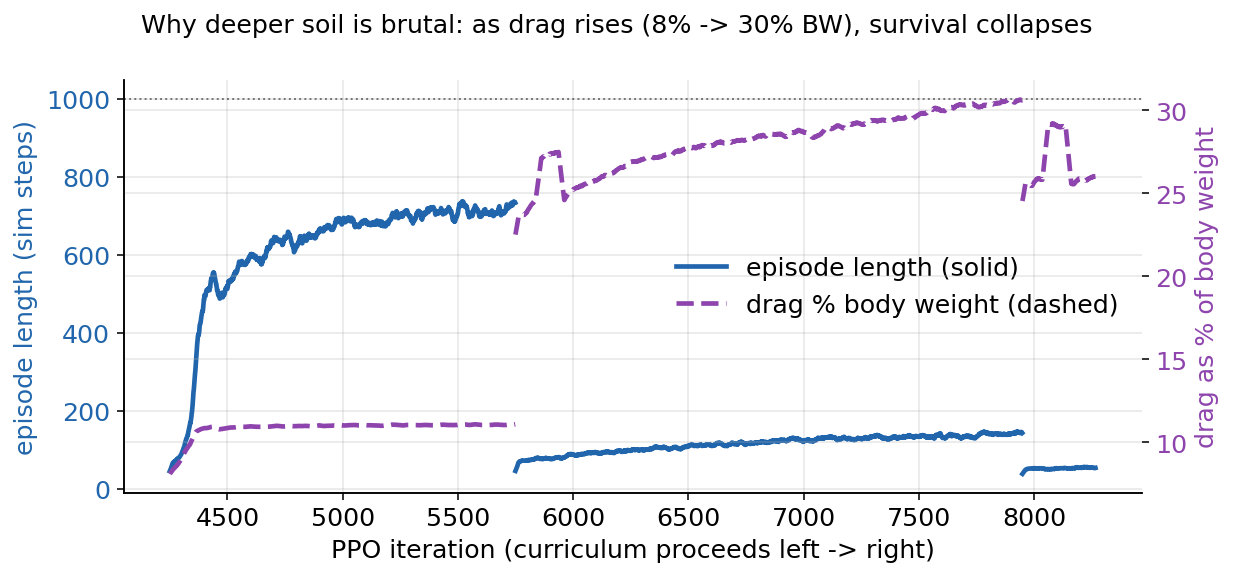
\includegraphics[width=0.84\textwidth]{fig4_difficulty.png}
  \end{center}
  \begin{itemize}\footnotesize
    \item As the curriculum deepens the soil, drag rises from $\sim$11\% to
          $\sim$25--30\% body weight (dashed).
    \item Survival (solid) \alert{collapses} from $\sim$730 steps to $\sim$50--150 ---
          a third of body weight in drag is more than the gait can absorb.
    \item This is why we report results on the mild/tuned regime, not full/wet soil.
  \end{itemize}
\end{frame}

\begin{frame}{Experiment 2: the result --- a clean null}
  \begin{center}
  \begin{tabular}{lccc}
    \toprule
    Eval on soil & DFH\_FULL & RIGID & Regret (DFH$-$RIGID) \\
    \midrule
    Tuned ($k{=}40$)     & 26.2\,s & 27.0\,s & \textcolor{bad}{$-0.8$\,s} \\
    De-saturated ($k{=}12$) & 27.6\,s & 31.4\,s & \textcolor{bad}{$-3.8$\,s} \\
    \bottomrule
  \end{tabular}
  \end{center}

  \vspace{0.8em}
  \begin{itemize}
    \item Rigid-trained policies \alert{matched or beat} soil-trained ones on the
          soil itself --- the opposite of the hypothesis.
    \item First suspect: the drag cap was saturating (clip 17--31\%), maybe hiding
          a real signal. So we \textbf{removed the confound} --- lowered $k$ until
          clipping fell to 3.2\%.
    \item The null got \emph{stronger}, not weaker ($-0.8 \rightarrow -3.8$\,s).
          The gap is real, not an artifact.
  \end{itemize}

  \vspace{0.4em}
  \begin{block}{Verdict \no}
    Soil-aware training did \textbf{not} produce a better soil walker.
    We report this as an honest negative result rather than overclaim.
  \end{block}
\end{frame}

\begin{frame}{Why we trust the null (and what \emph{did} work)}
  \begin{columns}[T]
    \begin{column}{0.5\textwidth}
      \textbf{The null is credible:}
      \begin{itemize}
        \item Negative control passed: DFH\_FULL beat SHUFFLED (+2.3\,s) --- the
              forces \emph{are} doing something coherent.
        \item Confound eliminated: clipping cut to 3.2\%, mean drag only
              $\sim$2.4\% body weight --- yet rigid still won.
        \item Trend is consistent across both dose levels.
      \end{itemize}
    \end{column}
    \begin{column}{0.5\textwidth}
      \textbf{The engineering succeeded:}
      \begin{itemize}
        \item DFH layer attaches \& runs live in IsaacSim, $120{\times}120$ grid,
              writeback every 4 steps.
        \item No measurable speed cost ($\sim$0.78\,s/iter).
        \item 27/27 unit + integration tests pass.
      \end{itemize}
      \vspace{0.4em}
      \footnotesize So the negative is a \emph{scientific} finding, not a broken
      pipeline.
    \end{column}
  \end{columns}

  \vspace{1em}
  \footnotesize Independent multi-round review scored the DFH \emph{claim} 3.0/10
  (evidence 2.0) and recommended pivoting to the honest null --- which is what these
  slides do.
\end{frame}

% ===============================================================
\begin{frame}{Takeaways}
  \begin{enumerate}
    \item \textbf{Furrow geometry is enough to deploy.} A staged curriculum on
          rigid plowed terrain gives a stable Hunter walker ---
          \texttt{mildsoil\_walker} powers the agri-field demo.
    \item \textbf{Deformable-soil training did not help.} Under a pre-registered,
          confound-controlled test, soil-aware policies did not beat rigid-trained
          ones on soil. Clean null.
    \item \textbf{The DFH simulator itself is solid} --- correct, fast, tested ---
          and remains a reusable IsaacLab extension for future, better-calibrated
          studies.
  \end{enumerate}

  \vspace{1.2em}
  \begin{center}
    \footnotesize Models: \texttt{huggingface.co/anhrisn/hunter-dfh-locomotion} \quad$\cdot$\quad
    Code: \texttt{extensions/dfh/}
  \end{center}
\end{frame}

\begin{frame}[plain]
  \begin{center}
    {\Large\textbf{Thank you}}\\[0.6em]
    Questions on the furrows curriculum or the DFH null welcome.
  \end{center}
\end{frame}

\end{document}
